The management structure can between companies based on their size and distribution. A company can have only one manager that tackles all the strategies from financial and to technical or it can have a hierarchy. 
The most generic hierarchy is described in \cref{sub-sec:levels}.
\subsection{Management levels}
\label{sub-sec:levels}
A generic hierarchy schema is usually based on 4 levels as in \cref{fig:levels}. The usual 
\begin{figure}[h]
\centering
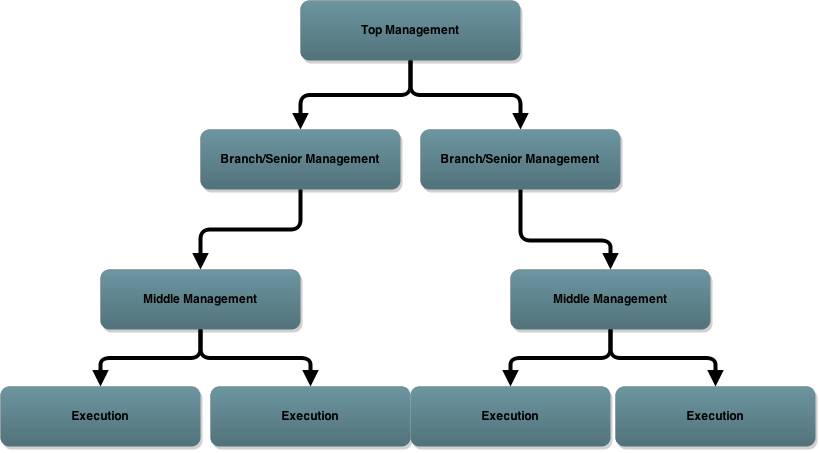
\includegraphics[width=0.8\textwidth]{img/levels.png}
\caption{Management Levels}
\label{fig:levels}
\end{figure}

\subsection{Management abilities}
\todo{Management abilities, Paraschiv notes}
\subsection{Management relationships}
\label{sub-sec:relationships}
\todo{small descriptions}

\subsubsection{People Manager - Direct Report}
\label{sub-sub-sec:pmdr}
\todo{You with your people} \newline

\subsubsection{People Manager - Upper Management}
\label{sub-sub-sec:pmum}
\todo{You with your bosses} \newline

